% !TEX encoding = UTF-8
% !TEX TS-program = pdflatex
% !TEX root = ../tesi.tex

%**************************************************************
\chapter{Gli assistenti virtuali}
\label{cap:assistenti-virtuali}
%**************************************************************

%\intro{Breve introduzione al capitolo}\\

%**************************************************************
\section{Premessa}
Un assistente virtuale è un software capace di interpretare il linguaggio naturale e dialogare con gli utenti che ne fanno uso, eseguendo determinati compiti. \\
Gli assistenti virtuali analizzati sono Assistant, Alexa e Siri e, nonostante siano software di tre aziende diverse, il loro funzionamento è molto simile: lo sviluppatore deve costruire un'abilità secondo principi molto simili, addestrare l'intelligenza che la costituisce e permettere all'utente di richiamarla. Queste abilità sono chiamate \emph{Action} per Assistant, \emph{Skill} per Alexa e \emph{Shortcuts} per Siri e sono caratterizzate da nome, frasi di richiamo e azioni da eseguire. \\
La prima proprietà in comune è meccanismo di funzionamento delle abilità: gli intenti. Essi consistono in un'azione che soddisfa una richiesta vocale effettuata da un utente e il servizio che la esegue, detto \emph{fulfillment}. \\
La seconda proprietà in comune è la possibilità di integrare all'interfaccia grafica quella grafica, ove possibile. Questo non viene trattato direttamente nell'analisi ma permetterà di giungere a conclusioni importanti nel seguito. \\
L'obiettivo dell'analisi riportata è presentare le sole funzionalità degli assistenti che sono state studiate, fornendo principi e metodi ad alto livello relativi a progettazione e implementazione; tuttavia non sono molto dettagliati perché ampiamente spiegati nelle pagine di documentazione.

%**************************************************************
\section{Assistant}
	\subsection{Introduzione}
	Assistant è l'assistente virtuale di Google ed è capace di riconoscere un comando vocale, elaborarlo attraverso un ragionamento e fornire una risposta. È una tecnologia in continuo miglioramento grazie anche all'immensa mole di dati che Google ha a disposizione per il suo addestramento.
	
	\begin{figure}[htbp]
		\begin{center}
			
\includegraphics[height=3cm]{logo-Assistant.png}
			\caption{Logo di Assistant}
		\end{center}
	\end{figure}
\pagebreak
	
	Reso pubblico dal 2016, Assistant è ora integrato in tutti i dispositivi con sistema operativo Android, a partire dalla versione 6.0 se hanno a disposizione almeno 1.5 GB di memoria \emph{\gls{ram}}\glsfirstoccur oppure dalla versione 5.0 se hanno a disposizione almeno 1 GB di memoria \emph{\gls{ram}}. È inoltre installabile nei dispositivi con sistema operativo iOS a partire dalla versione 10 e iPadOS; tuttavia l'integrazione è pessima in quanto per richiamarlo è necessario invocare Siri. Infine è fruibile nei dispositivi della linea Home e Nest di Google, costruiti e pensati appositamente per ottimizzarne le funzionalità.
	\subsection{Casi d'uso}
	\begin{itemize}
		\item dialogo con l'utente: \emph{Conversational Actions};
		\item integrazione di contenuti multimediali pensati per Assistant all'interno di pagine web: \emph{Content Actions};
		\item integrazione di Assistant nelle applicazioni Android per eseguire determinate funzionalità: \emph{App Actions};
	\end{itemize}
	\subsection{Conversational Actions}
		\subsubsection{Descrizione}
		Le \emph{Conversational Actions} estendono le funzionalità di Assistant con l'obiettivo di creare esperienze di conversazione personalizzate con gli utenti. Esse infatti permettono di gestire le richieste rivolte all'Assistente e le risposte costruite a seguito dell'elaborazione. Una caratteristica importante è la possibilità di comunicare con servizi Web o applicazioni esterne che forniscono una logica di conversazione aggiuntiva grazie agli appositi \emph{\gls{sdkg}}\glsfirstoccur.
		\subsubsection{Funzionamento}
		Il principio di funzionamento è illustrato nella seguente figura.
		\pagebreak
				
		\begin{figure}[htbp]
			\begin{center}
				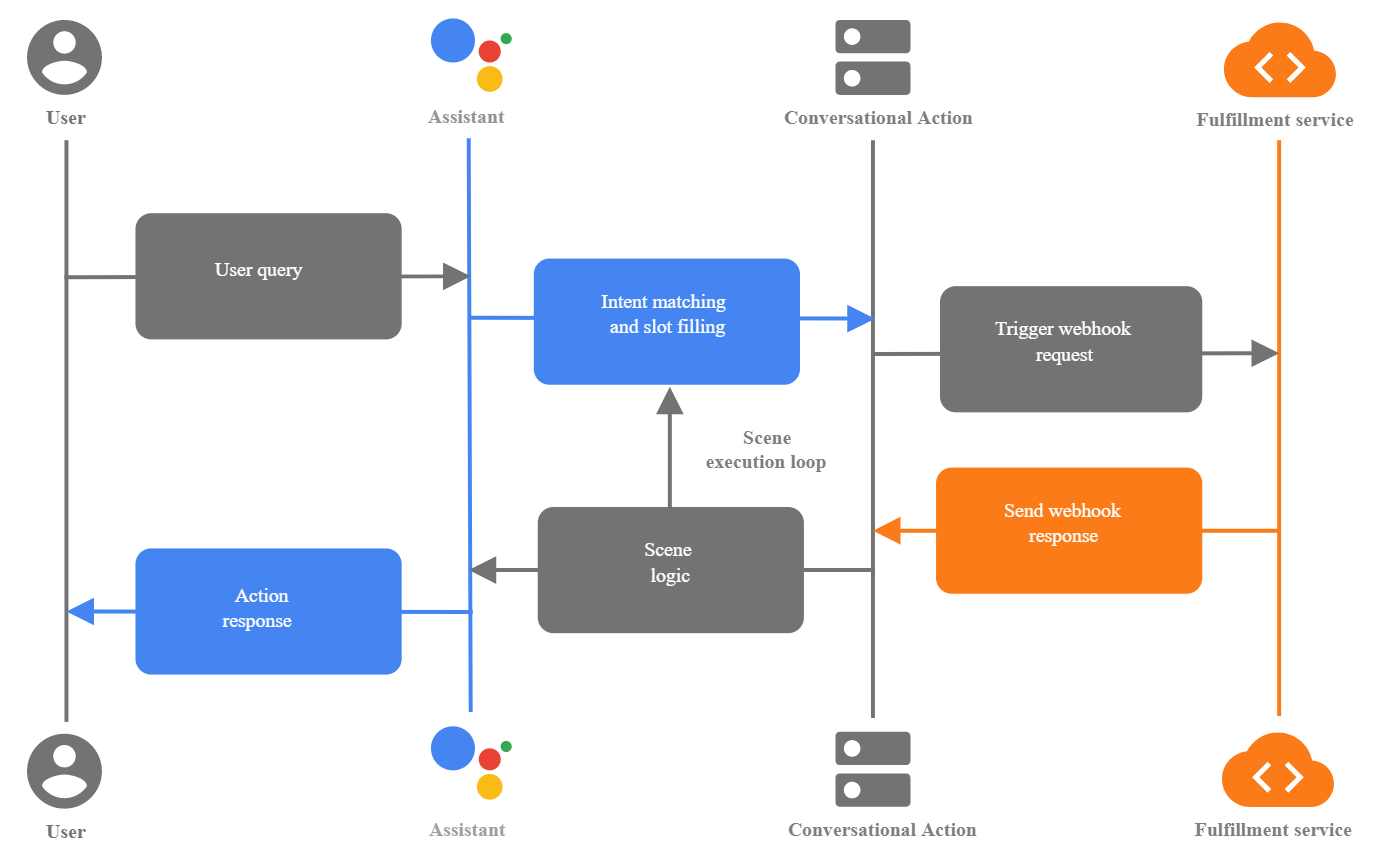
\includegraphics[height=9cm, width=\linewidth]{Assistant-conversation-fulfillment.PNG}
				\caption{Schema di funzionamento delle conversazioni con Assistant}
			\end{center}
		\end{figure}
%	\pagebreak
		
		Esso si articola quindi nei seguenti passi:
		\begin{enumerate}
			\item un utente lancia una richiesta sotto forma di comando vocale al dispositivo che ospita Assistant;
			\item il dispositivo esegue la porzione di software di Assistant che riconosce il comando vocale trasformandolo in stringhe di testo;
			\item il dispositivo invia la stringa riconosciuta ad un server remoto di Google, tramite protocollo \emph{\gls{httpg}S}\glsfirstoccur, dove risiede la \emph{\gls{nlug}} per l'elaborazione;
			\item la \emph{\gls{nlug}} del server remoto prova a verificare la possibile corrispondenza tra la stringa ricevuta e l'insieme di frasi che lo sviluppatore ha inserito durante la costruzione della propria abilità;
			\item se non vi è alcuna corrispondenza viene subito ritornata una risposta negativa e riferito all'utente. Si ricomincia quindi dal punto 1;
			\item se una corrispondenza ha dato esito positivo viene selezionato l'intento e attivato il suo servizio di \emph{fulfillment} che si occupa dell'esecuzione;
			\item la conclusione prevede il ritorno a cascata delle chiamate effettuate ed infine la costruzione e l'invio della risposta al dispositivo mittente;
			\item il dispositivo riferisce la riposta all'utente che potrà procedere con una nuova richiesta fino al termine dell'esecuzione dell'abilità configurato durante la costruzione oppure interrompere forzatamente la conversazione.
		\end{enumerate}
		Qualora l'utente effettuasse una richiesta invocazione, prima di scegliere l'intento da eseguire viene cercata una corrispondenza tra le \emph{Action} a disposizione per capire quale avviare.
		Infine, affinché la \emph{Action} tenga un comportamento adeguato, è necessario applicare correttamente i principi di costruzione e svolgere una consistente attività di addestramento durante lo sviluppo.
		%TODO: METTERE DEPLOY NEL GLOSSARIO 
		\subsubsection{Progettazione}
		Nella costruzione di una \emph{Action} la prima attività da svolgere è l'analisi dei requisiti ovvero comprendere dettagliatamente il comportamento che si vuole ottenere e non viene trattato in quanto di poco interesse per la ricerca. \\
		L'attività successiva, invece, è la progettazione ed è mirata a tre aspetti:
		\begin{itemize}
			\item modalità di invocazione;
			\item tipologia e formato delle richieste accettate;
			\item tipologia e formato delle risposte che l'utente si aspetta.
		\end{itemize}
		Per la progettazione di richieste e risposte è necessario ragionare sullo scopo dell'\emph{Action} che si vuole implementare e svolgere un'analisi statistica e probabilistica sulle frasi che l'utente potrebbe pronunciare o aspettarsi dall'assistente, cercando di rendere la conversazione più naturale possibile. Durante l'esecuzione della \emph{\gls{buildg}}\glsfirstoccur dell'\emph{Action}, Assistant sarà addestrato sulle frasi immesse al fine di interpretarle correttamente. \\
		Per la modalità di invocazione, invece, Google fa una distinzione:
		\begin{itemize}
			\item invocazione esplicita;
			\item invocazione implicita.
		\end{itemize}
		L'invocazione esplicita è la più comunemente utilizzata e consiste nell'esprimere una frase che riporti la seguente struttura:
		\begin{enumerate}
			\item parola di attivazione: "Hey Google" oppure "Ok Google";
			\item parola di avvio: chiedi, fai, dimmi, raccontami e vocaboli simili;
			\item nome di invocazione: nome deve identifica la \emph{Action};
			\item tips: parametri aggiuntivi, possibilmente opzionali, implementati come variabili che specificano ulteriormente la richiesta dell'utente;
			\item elementi aggiuntivi: l'utente può pronunciare parole aggiuntive con lo scopo di contestualizzare o precisare il dominio della richiesta.
		\end{enumerate}
		Grazie a questa struttura fissa, Assistant riesce a comprendere quale \emph{Action} attivare per avviare la conversazione. \\
		L'invocazione implicita, invece, si verifica quando l'utente effettua una richiesta senza aver esplicitato l'\emph{Action} o l'intento da eseguire. In questo caso la business logic di Assistant ha il compito di comprendere la richiesta e associare l'\emph{Action} che ritiene più corretta; qualora non ne trovasse alcuna, effettuerà una ricerca in Internet inserendo come testo la richiesta stessa e ritornerà i risultati come risposta. Tuttavia il funzionamento di questa modalità non è garantito da Google in quanto è ancora in via di sviluppo e richiede come condizione necessaria ma non sufficiente che lo sviluppatore abbia inserito un numero di frasi ampio e completo per l'addestramento.
		\subsubsection{Implementazione}
		L'attività che segue è l'implementazione e per svolgerla Google offre due strumenti:
		\begin{itemize}
			\item Dialogflow;
			\item Conversational Actions SDK.
		\end{itemize}
		Dialogflow è uno strumento utilizzato per creare conversazioni personalizzate in modo semplice ed intuitivo. Si basa sulla \emph{\gls{nlug}} di Assistant e si appoggia ad un \emph{webhook} per la gestione dei dati, \emph{\gls{firebaseg}}\glsfirstoccur è quello predefinito. \\
		Per costruire una \emph{Conversational Action} necessita un agente ovvero un modulo di comprensione del linguaggio naturale che gestisce le conversazioni con gli utenti sgravando lo sviluppatore di numerosi oneri; deve quindi essere creato prima di iniziare l'effettiva costruzione. A causa dei limiti imposti dall'account \emph{Firebase} disponibile non si è potuto approfondire il suo funzionamento come invece si è fatto per Alexa con uno strumento simile fornito da Amazon; tuttavia i principi di funzionamento e implementazione sono molto simili. \\
		Le Conversational Actions SDK consistono in un'interfaccia \emph{\gls{httpg}S} che permette di costruire ed eseguire le \emph{Conversational Actions} all'interno di una propria applicazione per elaborare le richieste effettuate ad Assistant. Grazie ad essa infatti Assistant può comunicare con applicazioni terze; il requisito che ne deriva è possedere una propria \emph{\gls{nlug}} per la comprensione del linguaggio naturale. L'architettura ad alto livello del sistema che rappresenta l'utilizzo delle \emph{Conversational Actions} attraverso \emph{\gls{sdkg}} è così composta:
		\begin{itemize}
			\item dispositivo fisico con Assistant integrato che riceve la richiesta vocale dell'utente;
			\item \emph{\gls{nlug}} di Google che ha il compito di riconoscere la richiesta dell'utente e associare l'intento corretto;
			\item servizio cloud remoto che, ricevuta la richiesta di esecuzione dell'intento, esegue il servizio di \emph{fulfillment} associato e ritorna la risposta alla \emph{\gls{nlug}} che a sua volta la ritorna al dispositivo.
		\end{itemize}
		%Segue un'immagine illustrativa dell'architettura.
		%TODO: INSERIRE IMMAGINE
		Le componenti di un agente di Dialogflow oppure una \emph{Conversational Actions} costruita con le \emph{\gls{sdkg}} sono uguali:
		\begin{itemize}
			\item Default Actions: azione cui corrisponde l'evento chiamato \textit{GOOGLE}\_\textit{ASSISTANT}\\ \_\textit{WELCOME} per Dialogflow e \textit{actions.intent.MAIN} per le \emph{\gls{sdkg}} che rappresenta la prima interazione con l'\emph{Action}; una condizione necessaria che la caratterizza è l'esistenza di uno ed un solo intento per gestire questo evento. La risposta predefinita è statica e preconfigurata ma è comunque possibile renderla dinamica costruendo un servizio di \emph{fulfillment} che la compone a tempo di esecuzione;
			\item Addictional Actions: azione aggiuntiva alla Default Actions utilizzata per aggiungere e specificare le capacità dell'\emph{Action} stessa. Possono essere molteplici e sono automaticamente indicizzate per l'invocazione implicita.
		\end{itemize}
		Ognuna di queste componenti corrisponde ad un intento che l'\emph{Actions} può gestire. \\
		Una volta stabilite queste componenti, è necessario definire l'interfaccia della propria conversazione. Per poterlo fare si deve creare un intento definendo:
		\begin{itemize}
			\item nome;
			\item contesto;
			\item evento scatenante;
			\item frasi di input per l'addestramento;
			\item azioni da eseguire;
			\item eventuali parametri aggiuntivi per la conversazione e formato della risposta.
		\end{itemize}
		Le azioni da eseguire corrispondono alla creazione di un \emph{fulfillment} che fornisce la logica per processare la richiesta dell'utente e generare una risposta. \\
		Qui emerge una grande differenza tra Dialogflow e \emph{\gls{sdkg}}: mentre il primo utilizza la \emph{\gls{nlug}} di Google rivelandosi quindi di poco interesse per i progetti dell'azienda, il secondo prevede l'utilizzo obbligatorio di una \emph{\gls{nlug}} proprietaria dello sviluppatore che invece si è rivelato utile per l'azienda.
		\subsubsection{Comunicazione}
		Lo scambio di dati tra il dispositivo che interagisce direttamente con l'utente e la \emph{\gls{nlug}} di Assistant avviene tramite oggetti JSON di cui però non viene fornita la struttura nella documentazione. \\
		Lo scambio di dati che invece avviene tra la \emph{\gls{nlug}} di Assistant e quella della proprio applicativo, diretta conseguenza dell'utilizzo delle \emph{\gls{sdkg}}, prevede un metodo di comunicazione dedicato. Google perciò impone l'utilizzo di oggetti JSON con una struttura fissata in cui campi dati più importanti sono:
		\begin{itemize}
			\item isInSandbox: attributo booleano, se vale true indica l'utilizzo in un ambiente di test;
			\item Surface: oggetto che contiene la modalità di interazione, scelta tra solo testuale, solo visiva e multimediale;
			\item Inputs: oggetto che contiene l'insieme degli input specificati per la \emph{Actions} tra cui la richiesta dell'utente sotto forma di stringa testuale;
			\item User: oggetto che contiene le informazioni dell'utente che ha eseguito la richiesta;
			\item Device: oggetto che contiene le informazioni del dispositivo da cui è arrivata la richiesta;
			\item Conversation: oggetto che contiene i dati strettamente legati alla conversazione in corso tra cui conversationId che la identifica univocamente e conversationToken che salva i dati durante la conversazione.
		\end{itemize}
		Di particolare rilevanza è il salvataggio dei dati durante la conversazione in quanto permette di avere sempre a disposizione determinati dati, possibilmente importanti, per la corretta esecuzione dell'\emph{Action} ma soprattutto di dare all'utente la sensazione di interagire con un sistema intelligente che ha capacità di memoria. Quest'ultima caratteristica è molto importante perché consente di definire e mantenere il contesto della conversazione, qualunque esso sia, incrementando notevolmente la qualità dell'esperienza d'uso. \\
		Per capire quali elementi devono essere salvati, Assistant utilizza delle variabili all'interno delle frasi di richiesta dette \emph{tips}. Esse sono definite dallo sviluppatore durante la progettazione e, quando l'utente pronuncia parole o dati in una posizione all'interno della frase corrispondente a quella di una variabile, vengono automaticamente salvati nel campo chiamato \emph{conversationToken}. Il loro limite è rappresentato dalla conversazione stessa: al termine tutti i dati salvati vengono persi. Perciò, se si vuole una persistenza duratura nel tempo, bisogna utilizzare un database.
	\subsection{Content Actions}
		\subsubsection{Descrizione}
		Le \emph{Content Actions} sono delle funzionalità basate su Assistant ma integrate nelle pagine Web. In particolare, inserendo dati strutturati al loro interno, permettono di costruire \emph{Actions} che ne presentano il contenuto in modo interattivo a seguito di un comando vocale.
		\subsubsection{Funzionamento}
		Il loro funzionamento verte esclusivamente sull'algoritmo di Google ed piuttosto semplice: l'utente esegue una ricerca in internet con un comando vocale lanciato ad Assistant e, se l'algoritmo di Google trova una \emph{Content Actions} che ha corrispondenza con la richiesta effettuata, il risultato sarà la risposta della \emph{Actions} stessa.
		\subsubsection{Dati strutturati}
		Le \emph{Content Actions} sono basate su dati strutturati. Essi corrispondono ad un oggetto JSON iniettato dinamicamente in una pagina \emph{\gls{html}} e contengono un insieme di metadati che definiscono le proprietà del contenuto multimediale che si vuole creare. Alcune di esse sono obbligatorie perché vengono utilizzate da Assistant per accedere al contenuto multimediale, molte altre sono opzionali ma consigliate per ottenere una migliore indicizzazione nel motore di ricerca. \\
		Esistono inoltre due formati alternativi agli oggetti JSON ma poco raccomandati:
		\begin{itemize}
			\item microdata: tag HTML che permette di includere dati strutturati al suo interno;
			\item RDFa: estensione di HTML5 che permette di definire contenuti per i motori di ricerca e in particolare per l'indicizzazione.
		\end{itemize}
		Sono messi a disposizione principalmente per compatibilità con sistemi che ne fanno uso.
		\subsubsection{Costruzione}
		Per costruire una \emph{Content Actions} è necessaria una progettazione mirata della pagina e a tal proposito Google offre un insieme di template pensati per le attività che più si prestano: podcasts ricette, news, \emph{How-to guides} e FAQs. \\
		Durante la realizzazione della pagina, invece, si devono inserire i dati strutturati in base alle proprie esigenze ed effettuare dei test per verificarne la corretta indicizzazione attraverso gli strumenti forniti da Google. \\
		È infine importante notare che Google non garantisce il richiamo della propria \emph{Actions} in nessuna condizione: l'algoritmo di ricerca, infatti, ha come obiettivo principale fornire all'utente i migliori risultati possibili nel momento in cui viene eseguita la ricerca e ciò può non corrispondere con la propria \emph{Actions}.
	\subsection{App Actions}
		\subsubsection{Descrizione}
		Le \emph{App Actions} sono delle funzionalità aggiuntive di Assistant che interagiscono esclusivamente con applicazioni Android ma sono ancora in via di sviluppo. In particolare permettono agli utenti di eseguire il \emph{deep linking} delle funzionalità specifiche di un'applicazione attraverso un comando vocale ed il loro risultato può manifestarsi sotto forma di risposta vocale oppure grafica, facendo opzionalmente uso delle \emph{Android Slides}.
		Infine è importante notare che le \emph{App Actions} sono per ora fornite in anteprima e supportano solo la lingua inglese americana.
		\subsubsection{Funzionamento}
		Il funzionamento delle \emph{App Actions} è rappresentato dalla seguente figura.
		
		\begin{figure}[htbp]
			\begin{center}
				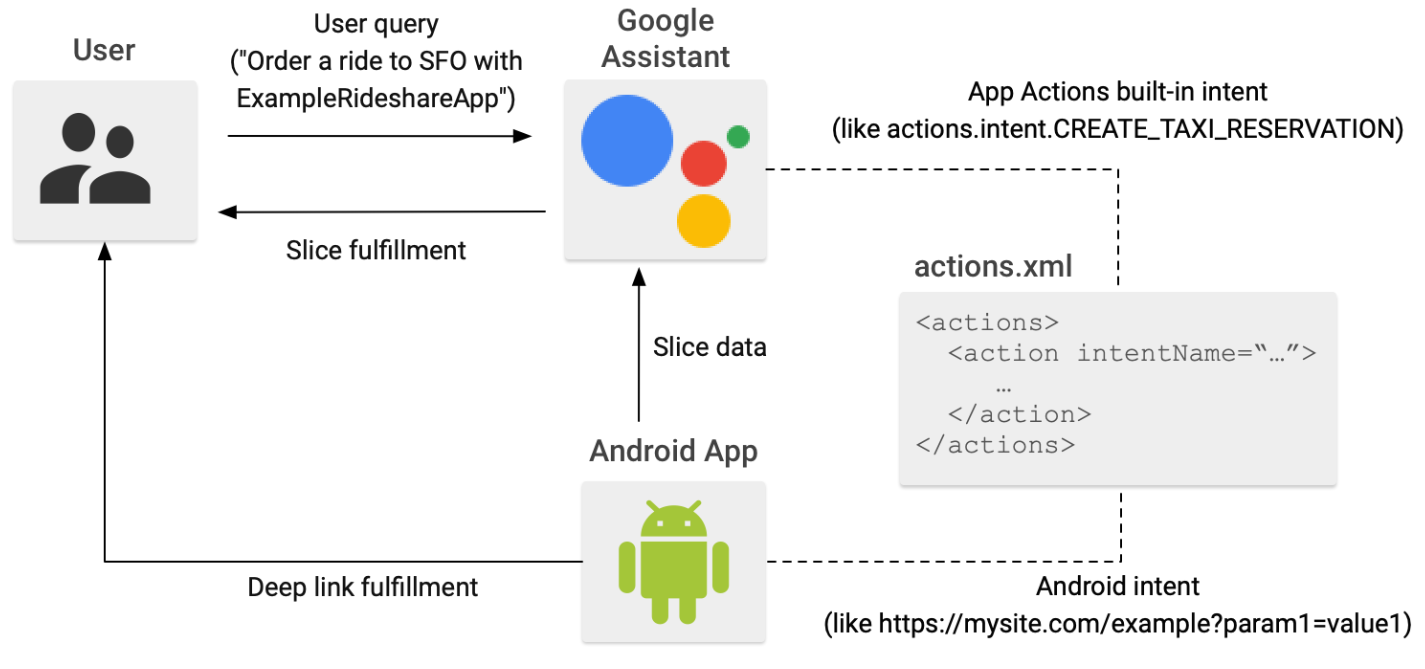
\includegraphics[height=6cm]{AppActions-funzionamento.PNG}
				\caption{Schema di funzionamento delle App Actions}
			\end{center}
		\end{figure}
		
		Viene descritto dai seguenti passi:
		\begin{enumerate}
			\item un utente invoca una \emph{App Actions} attraverso un apposito comando vocale;
			\item Assistant riconosce il comando vocale trasformandolo in stringhe di testo;
			\item il dispositivo invia la stringa riconosciuta ad un server remoto di Google, tramite protocollo \emph{\gls{httpg}S}, dove risiede la \emph{\gls{nlug}} per l'elaborazione;
			\item la \emph{\gls{nlug}} del server remoto prova a verificare la possibile corrispondenza tra la stringa ricevuta e la frase che lo sviluppatore ha predisposto per l'attivazione;
			\item se non vi è alcuna corrispondenza l'assistente eseguirà una ricerca in Internet della richiesta ritornando l'esito come risposta;
			\item se la corrispondenza ha dato esito positivo viene selezionato l'intento associato con il suo servizio di \emph{fulfillment} che si occupa dell'esecuzione;
			\item la conclusione prevede la risposta all'utente in termini di funzionalità eseguita.
		\end{enumerate}
		\subsubsection{Progettazione}
		La progettazione di \emph{App Actions} presuppone l'esistenza di un'applicazione costruita per Android a cui aggiungerla. Gli elementi cardine la decisione della frase di invocazione in quanto non è possibile averne solo una per ogni intento e rappresenta l'unica modalità di attivazione della \emph{Action} e la scelta dell'intento stesso in quanto deve essere il più adeguato a ciò che si vuole realizzare tra quelli possibili. Gli intenti disponibili sono solo quelli preconfigurati da Google e i macro argomenti che trattano sono:
		\begin{itemize}
			\item attivare funzionalità delle applicazioni;
			\item effettuare degli ordini online;
			\item operazioni in ambito finanziario;
			\item ordinare cibi e bevande da un menù preconfigurato;
			\item monitoraggio di salute e fitness;
			\item richiedere trasporto tramite Taxi.
		\end{itemize}
		Ad oggi non è ancora possibile costruire un intento personalizzato.
		\subsubsection{Implementazione}
		Dopo aver progettato la \emph{Action} si passa all'implementazione. Questa consiste nell'associare l'intento ed il suo \emph{fulfillment} all'applicazione. Più in dettaglio si deve:
		\begin{itemize}
			\item registrare il proprio intento nel file \emph{actions.xml} mappando gli eventuali parametri con il servizio di \emph{fulfillment} collegato;
			\item aggiornare il file \emph{AndroidManifest.xml} inserendo le dipendenze con gli intenti designati.
		\end{itemize}
		Dopo aver svolto questi compiti è necessario associare la \emph{Action} con il plug-in \emph{App Actions Test Tool} integrato in Android Studio ed eseguire almeno un test altrimenti non è possibile richiamarla.
	\subsection{Proof of concept}
		\subsubsection{Analisi dei requisiti}
		Per il proof of concept relativo ad Assistant, in comune accordo con il tutor e sulla base delle ricerche effettuate, è stato scelto di implementare una \emph{App Action} sull'argomento del fitness. Il suo scopo è verificare la fattibilità e le potenzialità delle \emph{App Action}, nonostante il loro attuale supporto alla sola lingua inglese, con un esempio concreto.
		Ho quindi deciso di realizzare un timer con un'interfaccia grafica minimale che calcoli il tempo impiegato nello svolgimento di attività fisica per ogni sport disponibile nei \emph{built-in intents}, con la possibilità di attivarlo tramite comando vocale.
		\subsubsection{Implementazione}	\mbox{}
		Nell'attività di implementazione ho seguito le linee guida fornite da Google. Inizialmente ho realizzato un'applicazione Android che presentasse tutte le funzionalità previste, fruibili tramite l'interfaccia grafica. Più in dettaglio l'utente può attivare il timer dall'apposito pulsante, fermare l'attività in qualunque momento e visualizzare i risultati nello storico. 
		
		\pagebreak
		
		\begin{figure}[htbp]
			\begin{center}
				
\includegraphics[height=6.1cm]{funzionamento AppActions.jpg}
				\caption{Esempio interfaccia PoC con Assistant}
			\end{center}
		\end{figure}
	
		A questo punto ho registrato gli intenti scelti nel file \emph{actions.xml} e aggiunte le dipendenze nel file \emph{AndroidManifest.xml} ed infine ho sviluppato il codice che deve essere eseguito al lancio del comando vocale.

		\subsubsection{Test}
		Per eseguire i test ho configurato il plug-in \emph{App Actions Test Tool} che permette di eseguire le verifiche su un dispositivo fisico, in quanto il supporto al simulatore non è ancora attivo, e di associare la mia \emph{Action} ad Assistant.
		
		\begin{figure}[htbp]
			\begin{center}
				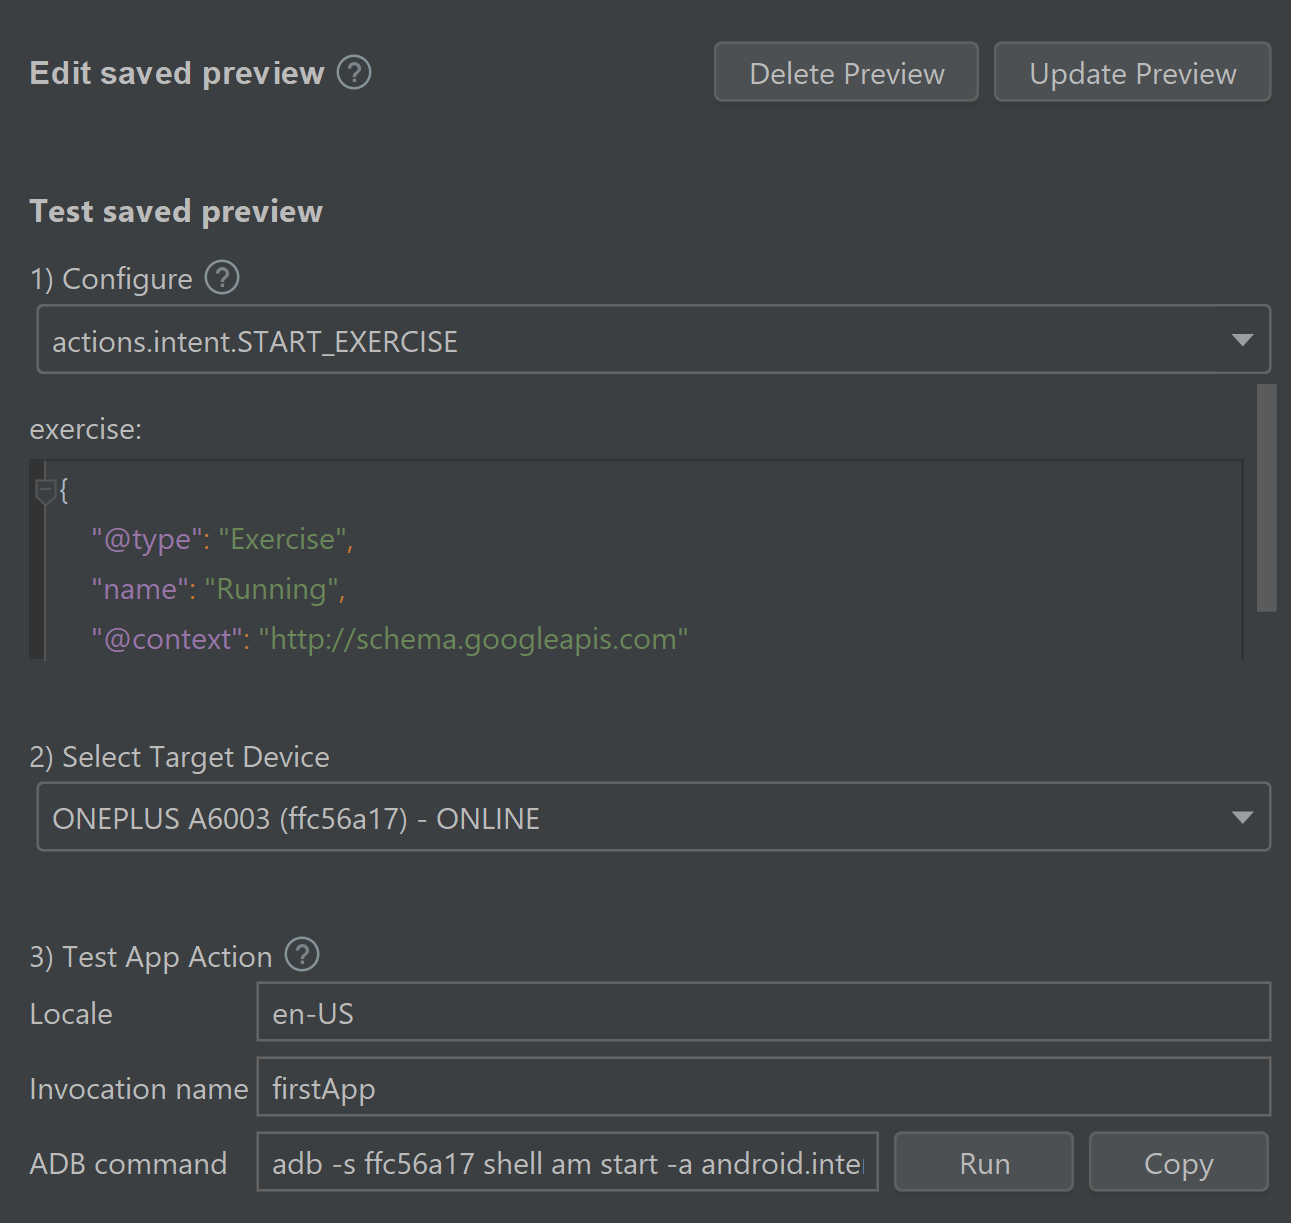
\includegraphics[height=7cm, width=8cm]{AppActionsTestTool.PNG}
				\caption{App Actions Test Tool}
			\end{center}
		\end{figure}
	\pagebreak
		
%**************************************************************
\section{Alexa}
	\subsection{Introduzione}
	Alexa è l'assistente virtuale di Amazon ed è capace di riconoscere un comando vocale, elaborarlo attraverso un ragionamento e fornire una risposta. È una tecnologia in continuo sviluppo grazie anche alla consistente mole di dati che Amazon ha a disposizione per il suo addestramento.
	
	\begin{figure}[htbp]
		\begin{center}
			
\includegraphics[height=3cm]{Alexa-logo.jpg}
			\caption{Logo di Alexa}
		\end{center}
	\end{figure}
	
	La prima versione di Alexa risale al 2014 e da allora ha fatto notevoli miglioramenti. È integrato in tutti i dispositivi della linea Echo di Amazon costruiti appositamente per ottimizzarne l'utilizzo; tuttavia è installabile in tutti i dispositivi con sistema operativo Android in versione 5.0 o maggiore, iOS in versione 9.0 o maggiore e iPadOS.
	\subsection{Casi d'uso}
	Il caso d'uso analizzato è: dialogo con l'utente attraverso le \emph{Skill}.
	\subsection{Skill di conversazione}
		\subsubsection{Descrizione}
		Le \emph{Skill} consistono in funzionalità personalizzate e aggiuntive per Alexa mirate a migliorare l'esperienza d'uso degli utenti. Attraverso le \emph{Skill} lo sviluppatore può ricevere le richieste rivolte ad Alexa, soddisfarle e restituire una risposta. Una caratteristica importante è la possibilità di comunicare con servizi Web o applicazioni esterne che forniscono una logica di conversazione aggiuntiva grazie alle \emph{\gls{apig}} presenti nell'Alexa Skill Kit. \\
		L'obiettivo principale delle \emph{Skill} è permettere all'utente una conversazione finalizzata a soddisfare un suo bisogno; tuttavia non è danno la possibilità di eseguire applicazioni o anche solo funzionalità al loro interno .
		\subsubsection{Funzionamento}
		Il principio di funzionamento si articola nei seguenti passi:
		\begin{enumerate}
			\item un utente lancia un comando vocale al dispositivo che ospita l'assistente;
			\item il dispositivo attiva un apposito elaboratore che riconosce le parole pronunciate trasformandole in stringhe di testo;
			\item il dispositivo manda la stringa riconosciuta ad un server remoto per l'elaborazione;
			\item il server remoto attiva la propria \emph{\gls{nlug}} che prova a cercare una corrispondenza tra la stringa ricevuta e l'insieme di frasi che lo sviluppatore ha inserito nella propria abilità;
			\item se la ricerca delle corrispondenze ha dato esito positivo viene selezionato l'intento;
			\item prima di eseguire il codice dell'intento vengono invocati gli eventuali \emph{Request Interceptors} definiti dallo sviluppatore, illustrati in un paragrafo successivo;
			\item viene richiamato gestore dell'intento, rappresentante il codice da eseguire, che porterà a termine l'intento;
			\item dopo aver gestito l'evento, vengono richiamati gli eventuali \emph{Response Interceptors} definiti dallo sviluppatore, illustrati in un paragrafo successivo;
			\item viene costruita la risposta e ritornata al dispositivo che ospita l'assistente;
			\item il dispositivo riferisce la riposta all'utente che potrà poi procedere con una nuova richiesta, fino al termine dell'esecuzione dell'abilità previsto dal programmatore durante la costruzione, oppure interrompere forzatamente la conversazione.
		\end{enumerate}
		\subsubsection{Progettazione}
		Nella costruzione di una \emph{Skill} la prima attività da svolgere è l'analisi dei requisiti ovvero comprendere dettagliatamente il comportamento che si vuole ottenere. L'attività successiva, invece, è la progettazione che deve essere mirata a tre aspetti:
		\begin{itemize}
			\item tipologia e formato delle richieste accettate;
			\item tipologia e formato delle risposte che l'utente si aspetta;
			\item modalità di invocazione.
		\end{itemize}
		Per la progettazione di richieste e risposte è necessario ragionare sullo scopo della \emph{Skill} che si vuole implementare e svolgere un'analisi statistica e probabilistica sulle frasi che l'utente potrebbe pronunciare o aspettarsi dall'assistente. L'obiettivo infatti è rendere la conversazione più naturale possibile. Durante l'esecuzione della \emph{\gls{buildg}} della \emph{Skill}, Alexa sarà addestrato sulle frasi immesse per interpretarle correttamente. \\
		Per la modalità di invocazione, anche Amazon fa una distinzione:
		\begin{itemize}
			\item invocazione esplicita;
			\item invocazione implicita.
		\end{itemize}
		L'invocazione esplicita è la più comunemente utilizzata e consiste nell'esprimere una frase che riporti la seguente struttura:
		\begin{enumerate}
			\item parola di attivazione: "Alexa";
			\item parola di avvio: chiedi, fai, dimmi, raccontami e vocaboli simili;
			\item nome di invocazione: nome deve identifica la \emph{Skill};
			\item slots: parametri aggiuntivi, possibilmente opzionali, implementati come variabili che specificano ulteriormente la richiesta dell'utente;
			\item elementi aggiuntivi: l'utente può pronunciare parole aggiuntive con lo scopo di contestualizzare o precisare il dominio della richiesta.
		\end{enumerate}
		Grazie a questa struttura fissa, Alexa è in grado di comprendere quale \emph{Skill} attivare per avviare la conversazione. \\
		L'invocazione implicita, invece, si verifica quando l'utente effettua una richiesta senza aver esplicitato la \emph{Skill} o l'intento da eseguire. In questo caso la business logic di Alexa deve comprendere la richiesta e associare la \emph{Skill} che ritiene più corretta; qualora non ne trovasse alcuna, effettuerà una ricerca in Internet inserendo come testo la richiesta stessa e ritornerà come risposta i risultati. Tuttavia il funzionamento di questa modalità non è garantito da Amazon in quanto è ancora in uno stato embrionale e richiede, come condizione necessaria ma non sufficiente, che lo sviluppatore abbia inserito un numero di frasi ampio e completo per l'addestramento.
		\subsubsection{Implementazione}
		L'attività che segue è l'implementazione. In merito a ciò Amazon offre due strumenti:
		\begin{itemize}
			\item Alexa Developer Console;
			\item Alexa SDK.
		\end{itemize}
		Il primo è Alexa Developer Console è uno strumento che integra Alexa Skills Kit e fornisce un'interfaccia allo sviluppare per creare \emph{Skill} personalizzate di diverse tipologie, tra cui quelle di conversazione, in modo semplice e intuitivo. Si basa sulla \emph{\gls{nlug}} di Alexa e si appoggia ad {AWS Lambda} come \emph{webhook} predefinito per la gestione dei dati. \\
		Per implementare una \emph{Skill} necessita di due macro compiti:
		\begin{itemize}
			\item costruire un modello di interazione;
			\item implementare la logica interna.
		\end{itemize}
		Costruire un modello di interazione significa definire l'interfaccia vocale e gli intenti che si vogliono implementare. Più in dettaglio si intende formalizzare ed inserire nell'interfaccia grafica le possibili frasi di invocazione, richiesta e risposta e gli eventuali slot. Con definizione degli intenti, invece, si intende formalizzare le azioni che la \emph{Skill} deve essere capace di eseguire. In particolare è possibile scegliere tra gli intenti \emph{built-in} ovvero quelli già preconfigurati da Amazon e quelli personalizzati, interamente a carico dello sviluppatore, dei quali è necessario definire:
		\begin{itemize}
			\item nome;
			\item contesto;
			\item evento scatenante;
			\item frasi di input per l'addestramento;
			\item azioni da eseguire;
			\item eventuali parametri aggiuntivi per la conversazione e formato della risposta.
		\end{itemize}
		Non ci sono vincoli sull'utilizzo di uno piuttosto che dell'altro e infatti possono anche essere usati contemporaneamente. \\
		%TODO:FORNIRE ALCUNI ESEMPI SE POSSIBILE
		Implementare la logica interna significa implementare il codice che definisce il comportamento dei singoli intenti e quindi della \emph{Skill} nel suo complesso. \\
		Il secondo strumento disponibile è \emph{Alexa SDK} e consiste a sua volta in un insieme di strumenti che permettono allo sviluppatore di interagire con Alexa da un'applicativo esterno che possiede una propria \emph{\gls{nlug}}. È disponibile nei linguaggi Javascript/Typescript, Java e Phyton. I principi di progettazione e implementazione sono gli stessi di quelli analizzati per Alexa Developer Console con la sola differenza che, utilizzando Alexa SDK, è necessario aggiungere uno strato di comunicazione per lo scambio di dati tra Alexa ed il proprio applicativo che avviene sotto forma di oggetti JSON.
		\subsubsection{Comunicazione}
		Lo scambio di dati tra il dispositivo che interagisce direttamente con l'utente e la \emph{\gls{nlug}} di Alexa avviene tramite oggetti JSON di cui però non viene fornita la struttura nella documentazione. \\
		Lo scambio di dati che invece avviene tra la \emph{\gls{nlug}} di Alexa e quella della proprio applicativo, diretta conseguenza dell'utilizzo delle \emph{\gls{sdkg}}, prevede un metodo di comunicazione dedicato. Amazon ha deciso di utilizzare gli oggetti JSON come mezzo per lo scambio di dati con strutture fissate ma differenti per richiesta e risposta. \\
		I campi principali dell'oggetto di richiesta sono:
		\begin{itemize}
			\item session: oggetto che fornisce informazioni riguardanti il contesto associato alla richiesta. È disponibile solo per conversazioni che non contengono contenuti multimediali;
			\item context: oggetto che fornisce le informazioni riguarrdanti lo stato della conversazione corso, del servizio di Alexa in esecuzione e del dispositivo con cui interagisce l'utente;
			\item request: oggetto che fornisce i dettagli della richiesta utente.
		\end{itemize}
		I campi principali dell'oggetto di risposta sono:
		\begin{itemize}
			\item sessionAttributes: mappa chiave-valore di tutti i dati di sessione;
			\item response: oggetto che definisce che cosa il dispositivo deve renderizzare per rispondere all'utente.
		\end{itemize}
		Di particolare rilevanza è il salvataggio dei dati durante la conversazione in quanto permette di richiedere determinati dati possibilmente importanti per la corretta esecuzione della \emph{Skill} ma soprattutto di dare all'utente la sensazione di interagire con un'intelligenza che ha capacità di memoria. Quest'ultima caratteristica è molto importante perché consente di definire e mantenere il contesto della conversazione, qualunque esso sia, incrementando notevolmente la qualità dell'esperienza d'uso dell'utente. \\
		Per capire quali elementi devono essere salvati, Alexa utilizza delle variabili all'interno delle frasi di richiesta dette \emph{slots}. Esse sono definite dallo sviluppatore durante la progettazione così che, quando l'utente pronuncia parole o dati in una posizione all'interno della frase corrispondente a quella di una variabile, vengono automaticamente salvati nel campo chiamato conversationToken. Il loro limite è rappresentato dalla conversazione stessa: al suo termine tutti i dati salvati vengono persi. Perciò, se si vuole una persistenza duratura nel tempo, bisogna utilizzare un database.
	\subsection{Proof of concept}
		\subsubsection{Analisi dei requisiti}
		Per il proof of concept relativo ad Alexa, in comune accordo con il tutor e sulla base delle ricerche effettuate, è stato scelto di implementare una \emph{Skill} in grado di riconoscere la data di nascita di una persona. Il suo scopo è verificare le capacità conversazionali di Alexa e comprendere il meccanismo di funzionamento da loro adottato con un esempio concreto oltre all'analisi teorica.
		Ho quindi deciso di realizzare un'interfaccia vocale in grado di comprendere un insieme di frasi preconfigurate per esprimere la propria data di nascita e un insieme di frasi per porre delle domande qualora l'utente fornisca una risposta incompleta o errata.
		\subsubsection{Implementazione}
		Per implementare la \emph{Skill} ho deciso di utilizzare la console fornita da Amazon e che maschera la complessità della \emph{\gls{sdkg}} e della comunicazione con essa. Il primo step è stato definire il modello di interazione composto da:
		\begin{itemize}
			\item frasi per la comunicazione con l'utente;
			\item intento per associare l'azione da eseguire;
			\item slot per le variabili.
		\end{itemize}
		Inizialmente è stato definito l'insieme delle frasi possibili per le richieste dell'utente e le risposte di Alexa. Successivamente è stato implementato un intento personalizzato identificato dal nome \emph{RegisterBirthdayIntent} in cui sono stati definiti gli slot della conversazione: giorno, mese e anno.
		
		\begin{figure}[htbp]
			\begin{center}
				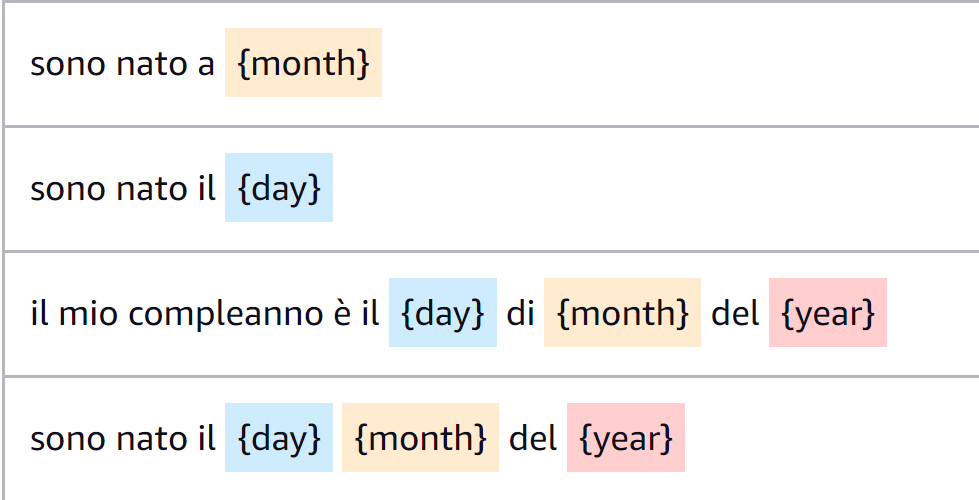
\includegraphics{AlexaIntent.PNG}
				\caption{Esempio frasi RegisterBirthdayIntent}
			\end{center}
		\end{figure}
		
		\mbox{}
		Infine è stato abilitato il meccanismo di richiesta degli slot in caso di mancanza. In questo modo, sulla base delle frasi che ho configurato, Alexa può continuare a chiedere all'utente giorno, mese e anno finché non saranno forniti.
		
		\begin{figure}[htbp]
			\begin{center}
				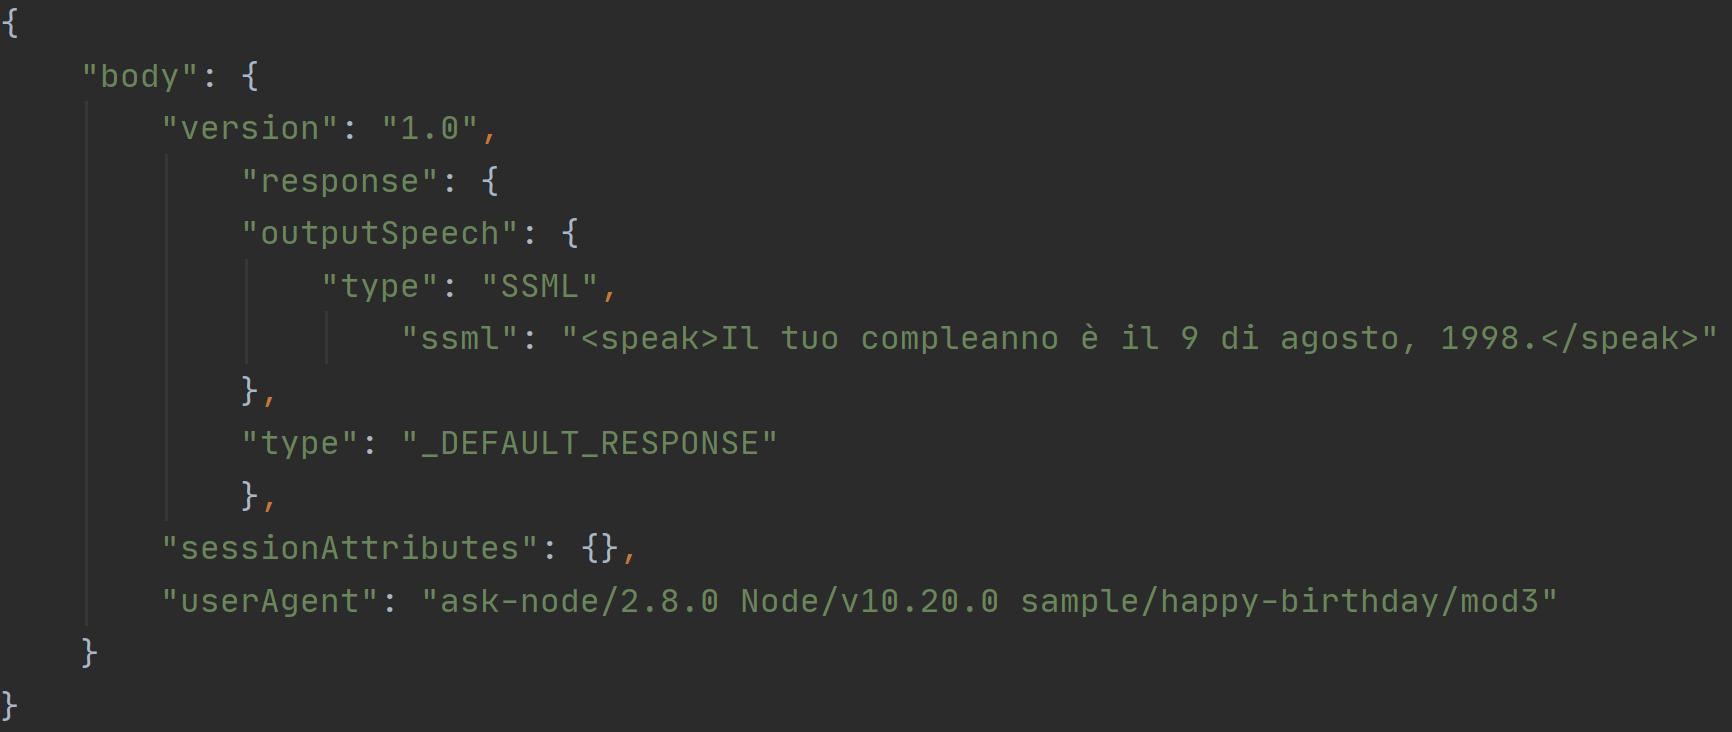
\includegraphics[width=\linewidth]{esempioJSONRisposta.PNG}
				\caption{Esempio JSON di risposta PoC Alexa}
			\end{center}
		\end{figure}
	
	\pagebreak
		
		\subsubsection{Test} \mbox{}
		Per eseguire i test è disponibile uno strumento all'interno della console che integra Alexa; tuttavia non ne permette l'automatizzazione.
		
		\begin{figure}[htbp]
			\begin{center}
				
\includegraphics[height=7cm]{funzionamentoPoCAlexa.PNG}
				\caption{Esempio funzionamento PoC Alexa}
			\end{center}
		\end{figure}
%**************************************************************
\pagebreak
\section{Siri}
	\subsection{Introduzione}
	Siri è l'assistente virtuale di Apple ed è capace di riconoscere un comando vocale, elaborarlo attraverso un ragionamento e fornire una risposta. È una tecnologia in continuo sviluppo grazie anche alla contingente mole di dati a disposizione di Apple per il suo addestramento.
	
	\begin{figure}[htbp]
		\begin{center}
			
\includegraphics[height=3cm]{logo-siri.png}
			\caption{Logo di Siri}
		\end{center}
	\end{figure}
	
	La prima versione è stata introdotta in iOS 5 nel 2012, senza ancora offrire il supporto a tutte le lingue e a tutti i dispositivi. Ora invece è integrato in Homepod e tutti i dispositivi con sistema operativo iOS versione 8.0 o superiore, iPadOS, watchOS, tvOS e MacOS versione 10.12 o superiore. Rimane comunque un esclusiva di Apple e non è installabile in altri sistemi.
	\subsection{Casi d'uso}
	Il caso d'uso analizzato è: esecuzione di operazioni specifiche nelle applicazioni attraverso le \emph{Shortcuts}.
	\subsection{Shortcuts}
		\subsubsection{Descrizione}
		Le \emph{Shortcuts} consistono in funzionalità aggiuntive per Siri e migliorano l'esperienza d'uso dei dispositivi da parte degli utenti. In particolare è possibile accedere all'applicazione \emph{Shortcuts} (comandi se le impostazioni sono in lingua italiana) e al suo interno, per ogni altra applicazione installata nel proprio dispositivo, sono visualizzate tutte le frasi messe a disposizione dagli sviluppatori per eseguire operazioni tramite Siri. L'utente può inoltre personalizzare tali frasi per renderle più intuitive e facili da ricordare. \\
		L'obiettivo principale delle \emph{Shortcuts} è migliorare e personalizzare l'interattività con le applicazioni dell'ecosistema Apple mentre l'aspetto conversazionale risulta finalizzato solo allo scopo principale.
		\subsubsection{Funzionamento}
		Il principio di funzionamento si articola nei seguenti passi:
		\begin{enumerate}
			\item un utente lancia un comando vocale al dispositivo che ospita Siri;
			\item il dispositivo attiva un apposito elaboratore che riconosce le parole pronunciate trasformandole in stringhe di testo;
			\item il dispositivo manda la stringa riconosciuta ad un server remoto per l'elaborazione;
			\item La \emph{\gls{nlug}} di Siri presente nel server remoto prova a cercare una corrispondenza tra la stringa ricevuta e l'insieme di frasi che lo sviluppatore ha inserito come \emph{Shortcuts} per la propria applicazione;
			\item se la ricerca della corrispondenza ha dato esito positivo viene selezionato l'intento;
			\item viene richiamata la porzione di codice che porterà a termine l'intento;
			\item viene costruita e ritornata la risposta al dispositivo che ospita l'assistente;
			\item il dispositivo riferisce la riposta all'utente che potrà procedere con una nuova richiesta fino al termine dell'esecuzione dell'abilità.
		\end{enumerate}
		\subsubsection{Progettazione}
		Nella costruzione di una Shortcut la prima attività da svolgere è l'analisi dei requisiti ovvero comprendere dettagliatamente il comportamento che si vuole ottenere. L'attività successiva, invece, è la progettazione che deve essere mirata a tre aspetti:
		\begin{itemize}
			\item tipologia e formato delle richieste accettate;
			\item tipologia e formato delle risposte che l'utente si aspetta;
			\item modalità di invocazione.
		\end{itemize}
		Per richieste e risposte è necessario ragionare sullo scopo della \emph{Shortcuts} che si vuole implementare e svolgere un'analisi statistica e probabilistica sulle frasi che l'utente potrebbe pronunciare o aspettarsi dall'assistente. In questo caso le frasi di richiesta assumono un importanza minore in quanto una delle funzionalità su cui Apple punta molto è fornire all'utente la possibilità di personalizzarle dall'applicazione \emph{Shortcuts}. L'obiettivo primario perciò si sposta dalla conversazione alla capacità di soddisfare un la richiesta dell'utente mentre assume un ruolo meno rilevante rendere la conversazione naturale. Durante l'esecuzione della \emph{\gls{buildg}} dell'applicazione, Siri sarà automaticamente addestrato sulle frasi immesse per interpretarle correttamente e di conseguenza verrà aggiornata \emph{Shortcuts}. \\
		Per la modalità di invocazione, anche Apple fa una distinzione:
		\begin{itemize}
			\item invocazione esplicita;
			\item invocazione implicita.
		\end{itemize}
		L'invocazione esplicita è la più comunemente utilizzata e consiste nell'esprimere una frase che riporti la seguente struttura:
		\begin{enumerate}
			\item parola di attivazione: "Hey Siri";
			\item parola di avvio: chiedi, fai, dimmi, raccontami e vocaboli simili;
			\item nome di invocazione: nome deve identifica la \emph{Shortcuts};
			\item parametri: parametri aggiuntivi, possibilmente opzionali, implementati come variabili che specificano ulteriormente la richiesta dell'utente;
			\item elementi aggiuntivi: l'utente può pronunciare parole aggiuntive con lo scopo di contestualizzare o precisare il dominio della richiesta.
		\end{enumerate}
		Grazie a questa struttura fissa, Siri è in grado di comprendere quale \emph{Shortcuts} attivare per avviare la conversazione. \\
		L'invocazione implicita, invece, si verifica quando l'utente effettua una richiesta senza aver esplicitato la Shortcut o l'intento da eseguire. In questo caso la business logic di Siri deve comprendere la richiesta e associare la \emph{Shortcuts} che ritiene più corretta; qualora non ne trovasse alcuna, effettuerà una ricerca in Internet inserendo come testo la richiesta stessa e ritornerà come risposta i risultati. Tuttavia il funzionamento di questa modalità non è garantito da Apple in quanto è ancora in uno stato embrionale e richiede, come condizione necessaria ma non sufficiente, che lo sviluppatore abbia inserito un numero di frasi ampio e completo per l'addestramento.
		\subsubsection{Implementazione}
		L'attività che segue è l'implementazione e in merito a ciò Apple offre uno strumento: Sirikit. Più in dettaglio è un insieme di strumenti che forniscono un'interfaccia per costruire interazioni tra Siri e le applicazioni. Le \emph{Shortcuts} si basano sulla \emph{\gls{nlug}} di Siri e prevedono l'utilizzo obbligatorio di Xcode in quanto devono essere inserite nel progetto designato per la loro integrazione. \\
		Apple è da sempre molto pignola in materia di autorizzazioni e sia per  l'utilizzo dei propri strumenti ma anche per il software. Quindi per implementare una \emph{Shortcuts} è prevista prima una serie di passaggi:
		\begin{itemize}
			\item abilitare la Capability di Siri nel proprio progetto di Xcode;
			\item configurare il file Info.plist includendo una chiave il cui valore è una stringa che descrive quali informazioni l'applicazione condivide con SiriKit;
			\item richiedere l’autorizzazione dell’applicazione iOS. Per farlo è necessario includere il metodo \emph{requestSiriAuthorization(\_:)} della classe INPreferences immediatamente dopo il codice che avvia l’applicazione. Grazie a ciò appare il prompt che fa scegliere all’utente se autorizzare o negare l’applicazione all’utilizzo di Siri. È comunque possibile cambiare tale scelta nelle impostazioni del dispositivo.
		\end{itemize}
		La maggior parte delle interazioni possibili tramite SiriKit è gestita dalle \emph{App Extension} ovvero estensioni delle funzionalità predefinite per un'applicazione sotto forma di intento. Queste si suddividono in due tipologie:
		\begin{itemize}
			\item \emph{Intent App Extension}: l’utente effettua una richiesta, essa viene ricevuta dall’applicazione che successivamente seleziona l’intento corretto per soddisfarla;
			\item \emph{Intent UI App Extension}: consiste in un \emph{intent App Extension} come la precedente in cui però, dopo aver soddisfatto la richiesta dell’utente, visualizza i contenuti in una finestra personalizzata. È un arricchimento non obbligatorio che si pone l’obiettivo di migliorare ll'esperienza d'uso dell'utente.
		\end{itemize}
		Il principio di costruzione è uguale per entrambe con l'ovvia differenza che per la seconda è necessario provvedere ad un'interfaccia grafica aggiuntiva. I passi sono quindi i seguenti:
		\begin{itemize}
			\item verificare che il procedimento di autorizzazione sia stato eseguito correttamente. Questo è possibile farlo controllando tramite Xcode che la Capability di Siri sia abilitata;
			\item aggiungere un \emph{Intents App Extension} (o \emph{Intent UI App Extension}) al progetto dal menu File > New > Target;
			\item specificare gli intenti supportati dall’Extension scelta all’interno del file Info.plist;
			\item scegliere dove salvare le proprie risorse. per farlo è opportuno utilizzare un container condiviso (scelta consigliata) oppure costruire un proprio servizio in un framework privato;
			\item creare tante classi handler quanti sono gli intent che si vogliono gestire e definire le operazioni da svolgere al loro interno;
			\item eseguire i test con procedura fornita da Xcode per le applicazioni iOS.
		\end{itemize}
		Per quanto rigurarda l'aggiunta degli intenti anche Apple, come i suoi competitori, fa una distinzione:
		\begin{itemize}
			\item \emph{System intents}: intenti di sistema preconfigurati da Apple;
			\item \emph{Custom intents}: intenti che lo sviluppatore costruisce e personalizzare in base alle sue esigenze.
		\end{itemize}
		
		I \emph{System intents} rappresentano le azioni più comunemente eseguite e prevedono un flusso di conversazione, opportunamente addestrato e testato, per il quale le app di sistema forniscono tutti i dati previsti. \\
		I \emph{Custom intents}, a differenza dei precedenti, permettono agli sviluppatori di creare degli intenti personalizzati in aggiunta ai System intents. Si deve quindi definire il proprio flusso di conversazione inserendo le possibili frasi di invocazione e di risposta. \\
		In entrambi le tipologie la gestione dell’apprendimento di nuove frasi è privilegiata lato utente perché può inserirle nell'applicazione Shortcuts; tuttavia è possibile delegare questo compito alla business logic di Siri ma è una funzionalità ancora allo stato embrionale. Inoltre, qualora si utilizzassero le \emph{Intents UI App Extension}, lo sviluppatore può implementare una grafica personalizzata senza vincoli alcuni. \\
		Le modalità per costruire gli intenti sono riassunte nei seguenti passaggi:
		\begin{itemize}
			\item aggiungere un Intent Definition File nell’App Target;
			\item definire il proprio intento sulla base delle funzionalità che si vuole implementare;
			\item definire gli eventuali parametri (vedi sezione Gestione della comunicazione);
			\item aggiungere i metadati e i Siri Dialog Data alla propria conversazione;
			\item definire le gerarchie tra i parametri (opzionale e poco utilizzato);
			\item definire le eventuali e possibili shortcuts che l’utente può aggiungere dall'apposita applicazione;
			\item creare e settare le frasi di richiesta e risposta.
		\end{itemize}
		Infine Apple non fornisce delle \emph{\gls{sdkg}} che permettano di realizzare quanto illustrato all'interno di un progetto che possieda una propria \emph{\gls{sdkg}}.
		\subsubsection{Comunicazione}
		Dato che lo scopo principale delle \emph{Shortcuts} che Apple mette a disposizione non è costruire delle conversazioni, è stato deciso di non approfondire il metodo di comunicazione che utilizza. Tuttavia è noto che, come per gli altri assistenti, è possibile inserire dei parametri corrispondenti a variabili all'interno delle frasi che vengono storicizzati affinché la \emph{Shortcuts} non venga portata a termine.
	\subsection{Proof of concept}
	Come \emph{\gls{pocg}} è stato pensato di costruire un'applicazione che consentisse l'esecuzione di un ordine di alimenti e quindi di aggiungere una Shortcut che inviasse l'ordine tramite Siri. Per problemi di licenze nell'account sviluppatore di Apple non è stato possibile collegare l'applicazione a Siri e quindi l'applicazione.

%**************************************************************
\section{Trattamento dei dati}
Per quanto concerne il trattamento dei dati che vengono scambiati durante l'esecuzione delle abilità, gli assistenti virtuali operano in modo del tutto simile. \\
Tutti i dispositivi che integrano un assistente virtuale rimangono sempre in ascolto di qualsiasi parola pronunciata in modo da essere reattivi qualora venga lanciata una parola di attivazione che richiami la loro attenzione. Tuttavia solo le parole recepite dall'attivazione alla conclusione di un'abilità vengono elaborate mentre le altre non sono considerate. Questo accade perché le aziende riceverebbero una mole di dati troppo elevata per essere processata, le reti per la connessione sarebbero intasate ma soprattutto gli utenti subirebbero una violazione di privacy. \\
Infine per garantire sicurezza durante lo scambio dei dati utilizzano il meccanismo \emph{\gls{authg}}\glsfirstoccur per l'autenticazione ed il protocollo \emph{\gls{httpg}S} che aggiunge uno strato di crittografia.
%**************************************************************
\section{Risultati}
In questa sezione vengono riportati i risultati salienti della ricerca svolta. Nella seguente tabella è presentato un confronto tra le funzionalità ad alto livello dei tre assistenti che sono state più rilevanti per lo stage.
\begin{table}
	\begin{tabularx}{\textwidth}{|X|X|X|X|}
		\hline
		\textbf{Funzionalità} & \textbf{Assistant} & \textbf{Alexa} & \textbf{Siri} \\\hline
		
		Creazione di conversazioni personalizzate & Supporto tramite \emph{Conversational Actions} sia con le \emph{\gls{sdkg}} sia con Dialogflow.  & Supporto tramite \emph{Skill} sia con le \emph{\gls{sdkg}} sia con Alexa Developer Console. & Funzionalità non supportata. \\
		\hline
		Integrazione nelle pagine Web & Supporto tramite \emph{Content Actions}. & Funzionalità non supportata. & Funzionalità non supportata. \\
		\hline
		Integrazione nelle applicazioni & Supporto tramite \emph{App Actions} solo su applicazioni Android. & Funzionalità non supportata. & Supporto tramite \emph{Shortcuts} solo su applicazioni dell'ecosistema Apple. \\
		\hline
	\end{tabularx}
	\caption{Tabella di confronto tra gli assistenti virtuali}
\end{table}
Nello sviluppo di abilità mirate alle conversazioni gli assistenti virtuali di Google e Amazon offrono rispettivamente strumenti molto simili come struttura e funzionalità offerte. \\
Apple e Google rientrano nel mercato di dispositivi quali computer, smartphone e tablet e si pongono l'obiettivo di migliorare l’interazione degli utenti con i propri prodotti offrendo la possibilità di creare abilità personalizzate all'interno delle proprie applicazioni. La differenza principale risiede nelle lingue supportate in quanto Apple fornisce il supporto a tutte le lingue in cui Siri è disponibile mentre Google per ora solo in inglese. \\
Infine Google è l'unico ad offrire l'integrazione di Assistant nell'interazione con le pagine Web. \\
In generale ho riscontrato che gli assistenti virtuali attuali sono pensati per un utilizzo di breve durata perciò è molto importante progettare le loro abilità seguendo questo principio per dare agli utenti un'esperienza d'uso migliore.
Oltre all'analisi delle funzionalità ho analizzato l'intelligenza degli assistenti e ho trovato i risultati di un test svolto su di essi in questo ambito che consiste nel verificare quale assistente è in grado di comprendere e rispondere correttamente al maggior numero di domande su un campione di 800.

\begin{figure}[htbp]
	\begin{center}
		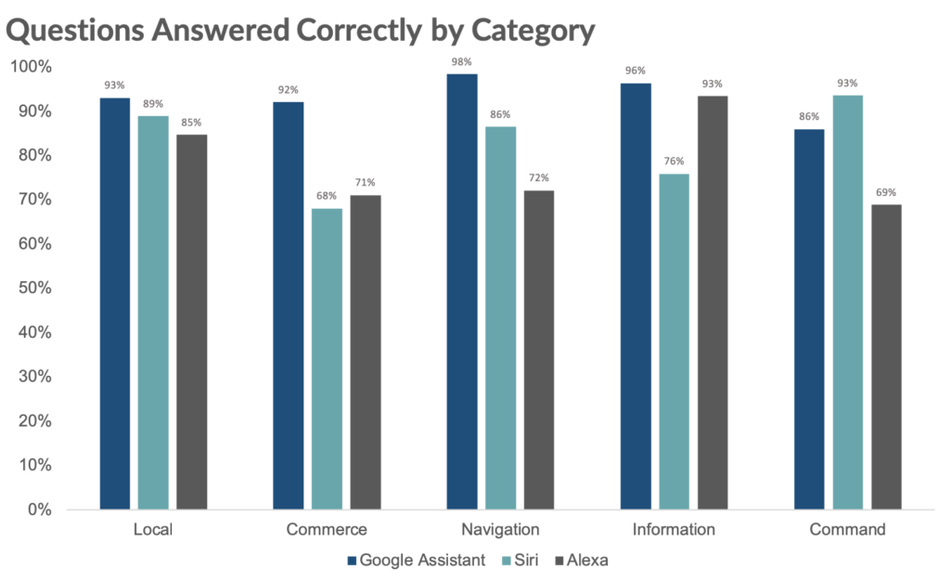
\includegraphics[height=8cm, width=\linewidth]{diagramma_confronto_assistenti.png}
		\caption{Diagramma di confronto nell'intelligenza degli assistenti}
	\end{center}
\end{figure}


Come si può vedere dal diagramma, l'esito è stato a favore di Google con un netto vantaggio. \\
Dunque da questa ricerca è emerso come Google fornisca un insieme più completo di funzionalità per il proprio assistente e come l'intelligenza che lo caratterizza sia superiore a quella degli altri probabilmente per la cospicua quantità di dati di varie categorie che ha a disposizione. 
%TODO:INSERIRE LE CONCLUSIONI
